\scanpage{40}
\mspage{39}
% Top proposition and three conditions, with inserted c).
\uline{Proposition} Pour tout $n\geq1$, soit $A_n\subset H^*(X^n)$ un \unsure{ss-vectoriel} \uline{stable} \inserted{par \uline{grp sym.}}.
Conditions équivalentes:

\unsure{(i)} a) Pour tout \deleted{$u\in H^*$} $u\in A_{n+m}\subset H^*(X^n\times X^m)$ et $x\in A_n\in H^*(X^n)$, on a $u(x)\in H^*(X^m)$.

b) Si $x\in A_n$, $y\in A_m$, alors $x\otimes y\in A_{n+m}$; pour tt $n$, $1\in A_n$.

\inserted{c) Pour \unsure{tte|toute} surjection $[1,n+1]\longrightarrow[1,n]$, son graphe dans $H^*(X^n\times X^{n+1})\in A_{2n+1}$. \unsure{Et $=$ chose pour tte injection|Et de même pour tte injection} $[1,n]\unsure{\lhook\joinrel\relbar|\subset}[1,n+1]$}

\unsure{(ii)} Les \deleted{\unsure{systèmes de}} $A_n$ sont des \uline{sous-algèbres}, stables par images inverses \inserted{et images directes} par \uline{projections} $X^{n+1}\longrightarrow X^n$, et \deleted{par images inverses} par images directes par injections $X^n\unsure{\lhook\joinrel\relbar|\hookrightarrow}X^{n+1}$.

\figure{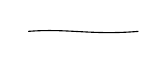
\begin{tikzpicture}\draw (0,0) .. controls (.5,.04) and (.8,-.05) .. (1.4,0);\end{tikzpicture}}

Ces conditions impliquent que les $A_n$ sont stables par ttes images inv. et images dir. par tte application simpliciale \inserted{$X^n\longrightarrow X^m$}, et que \deleted{\unsure{$A_n$}} pour tte telle application, $H^*(X^n\times X^m)$ \unsure{cont.} la classe du graphe\ldots

% Lower paragraph.
(iii) \unsure{Considérons} $A_{n+m}\in H^*(X^n\times X^m)$ comme un ens d'hom de $H^*(X^n)$ en $H^*(X^m)$, on veut que ces ens. soient stables par composition $(n,m\geq0)$, contiennent les identités, soient stables par $\unsure{\boxtimes|\otimes}$, et contiennent les hom images inverses et directes par une application simpliciale.
